%%%%%%%%%%%%%%%%%%%%
%
% $Beschreibung: Hier sind alle Informationen zu den Konstruktionsaufgaben zusammengefasst $
% $Autor: Theilmann $
% $Datum: 09.06.2024 $
% $Pfad: DemonstratorSchrittmotor/DeveloperDoc/Contents/de/Konstruktion.tex $
% $Version: 2 $
%
%
%%%%%%%%%%%%%%%%%%%

\chapter{Konstruktion}

In diesem Kapitel wird die Konstruktion des Demonstrator-Schrittmotors beschrieben. Zunächst werden die Rahmenbedingungen erläutert, anschließend werden das Gehäuse und die Anbauteile des Aluprofils besprochen. Abschließend wird die gesamte Baugruppe betrachtet.

\section{Rahmenbedingungen}

Das Gehäuse sowie sämtliche Anbauteile sollen mittels additiver Fertigung aus Polylactic Acid (PLA) hergestellt werden. Im und am Gehäuse werden sämtliche Komponenten zur Bedienung und Steuerung des Demonstrators untergebracht. Die Konstruktion soll eine komfortable Handhabung ermöglichen und sicherstellen, dass die Komponenten, wie beispielsweise das Tiny Machine Learning Shield mit dem aufgesteckten Arduino, fest sitzen.

\section{Arbeiten mit SolidWorks 2023}

Zur Herstellung des Gehäuses muss ein 3D-Modell mittels Computer Aided Design (\ac{cad}) erstellt werden. Hierfür wurde die Software SolidWorks 2023 vom französischen Software-Entwicklungsunternehmen Dassault Systèmes (DS) verwendet. \glqq \textit{SOLIDWORKS ist eine professionelle und leistungsstarke \ac{cad}-Software, die vor allem im Maschinenbau viel genutzt wird.}\grqq \cite[S.225]{Weber.2024} Für die Additve Fertigung muss das \ac{cad}-Modell als STL-Datei gespeichert werden. 

\section{Gehäusekonstruktion}

Zu Beginn wurden die Abmessungen der einzelnen Komponenten ermittelt, um die Dimensionen des Gehäuses festzulegen. Das Gehäuse, ersichtlich in Abbildung \ref{GehK}, besteht aus sechs Einzelteilen, die mit Innensechskantschrauben DIN 912 M3 verbunden werden.
	\begin{figure}[H]	
	 	\begin{center}
			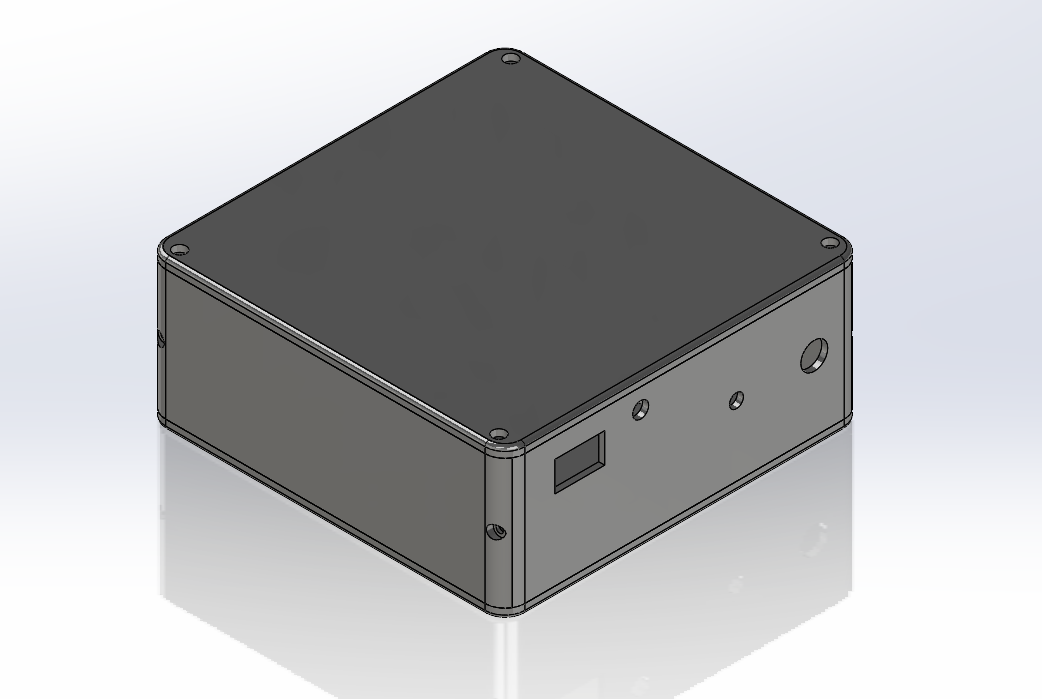
\includegraphics[width=\textwidth]{Images/Konstruktion/GehaeuseK.png}
			\caption{Baugruppe Gehäuse (Eigenaufnahme)} \label{GehK}
		\end{center}
	\end{figure}

Die Basis der Baugruppe ist die Bodenplatte mit einer Länge von 180 \ mm, einer Breite von 180 \ mm und einer Dicke von 7 mm, wie in Abbildung \ref{BodenK} dargestellt. An der Bodenplatte werden die anderen Teile des Gehäuses, das Schaltnetzteil, das Tiny Machine Learning Shield, das Aluminiumprofil, die Schrittmotorsteuerung und die Halterung für den Spannungswandler befestigt. Die Ecken sind mit einem Radius von 10 \ mm abgerundet. Die Bohrungen 1 bis 6 sind in Tabelle \ref{BohrungenGK} aufgeführt.

	\begin{figure}[H]
		\begin{center}
			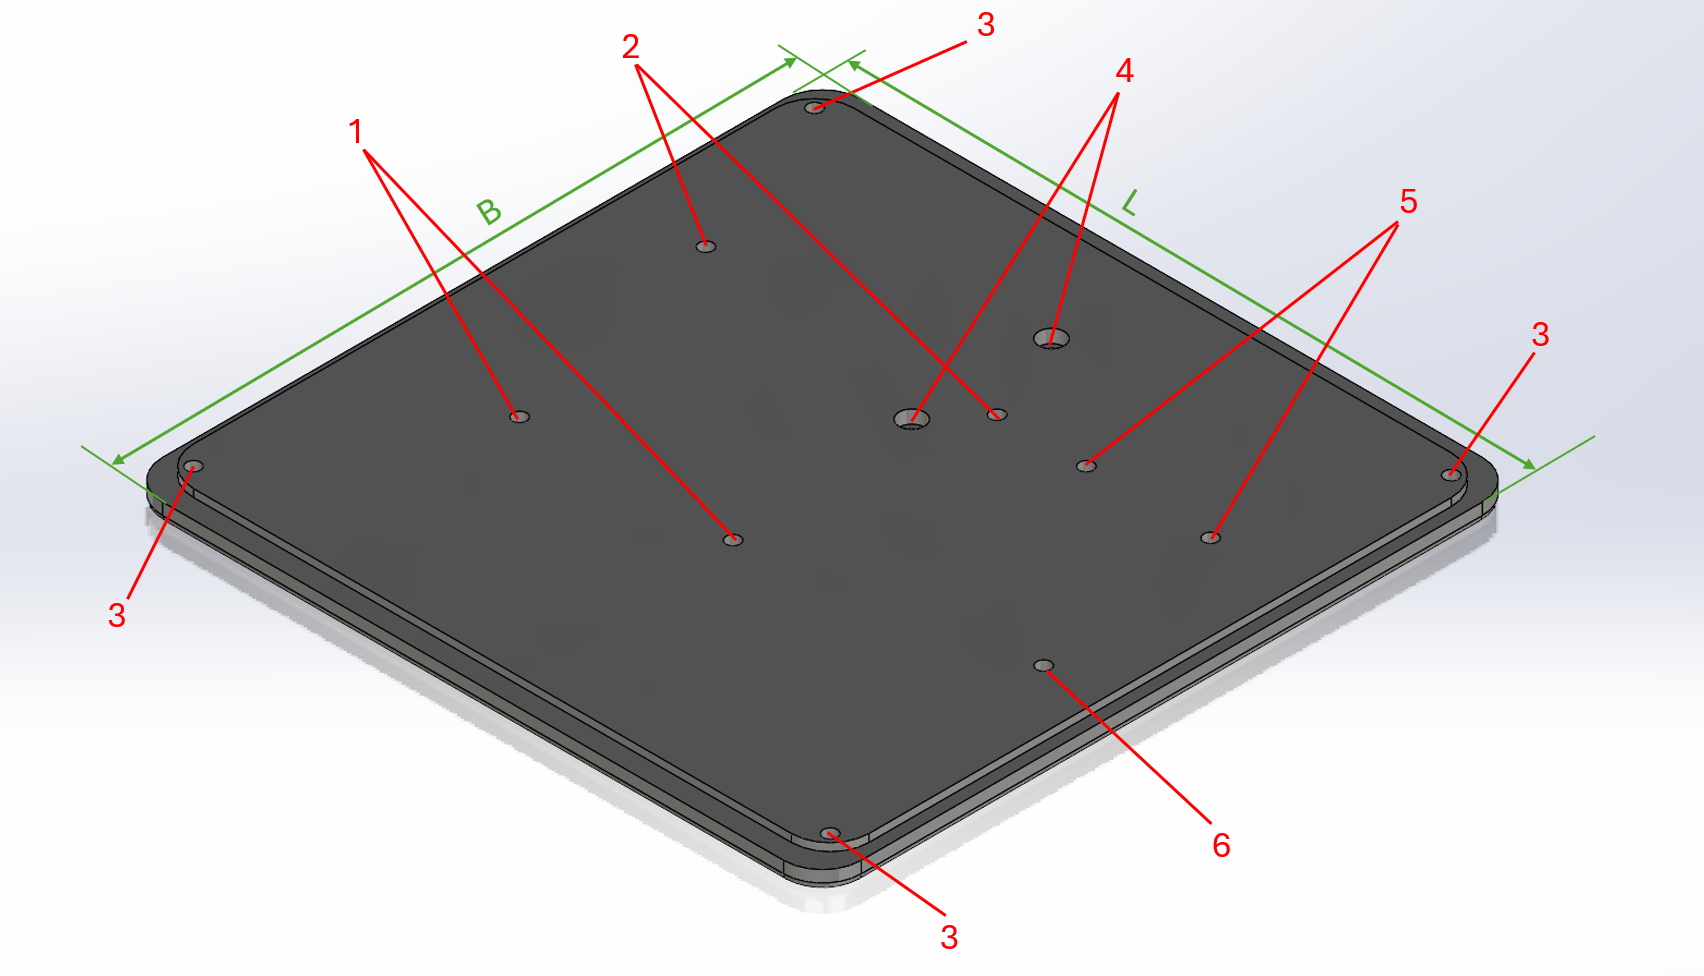
\includegraphics[width=\textwidth]{Images/Konstruktion/BodenK.png}
			\caption{Bodenplatte (Eigenaufnahme)} \label{BodenK}
		\end{center}
	\end{figure}

An der Bodenplatte wird die Vorderplatte befestigt. Sie hat eine Breite von 170 \ mm und eine Höhe von 65 \ mm, wie in Abbildung \ref{VorneK} dargestellt. Das OLED-Display wird von innen eingesetzt und mit DIN 912 M3$\times$6 Schrauben verschraubt (siehe Markierung a $25 \times 15 \ mm$  in Abb.\ref{VorneK}). Die LED wird von innen eingesetzt und mittels Presspassung fixiert (siehe Markierung b \O $ \ 8 \ mm$ in Abb.\ref{VorneK}). Der Drehwinkel-Encoder wird von innen durchgeführt und mittels einer P4-Mutter befestigt (siehe Markierung c \O $ \ 7 \ mm$  in Abb.\ref{VorneK}). Der Drucktaster wird von außen durchgeführt und mittels Kontermutter befestigt (s. Markierung a \O $ \ 13,5 \ mm$  in Abb.\ref{VorneK}). Die Bohrungen 7 bis 9 sind der Tabelle \ref{BohrungenGK} aufgeführt.  


	\begin{figure}[H]
		\begin{center}
			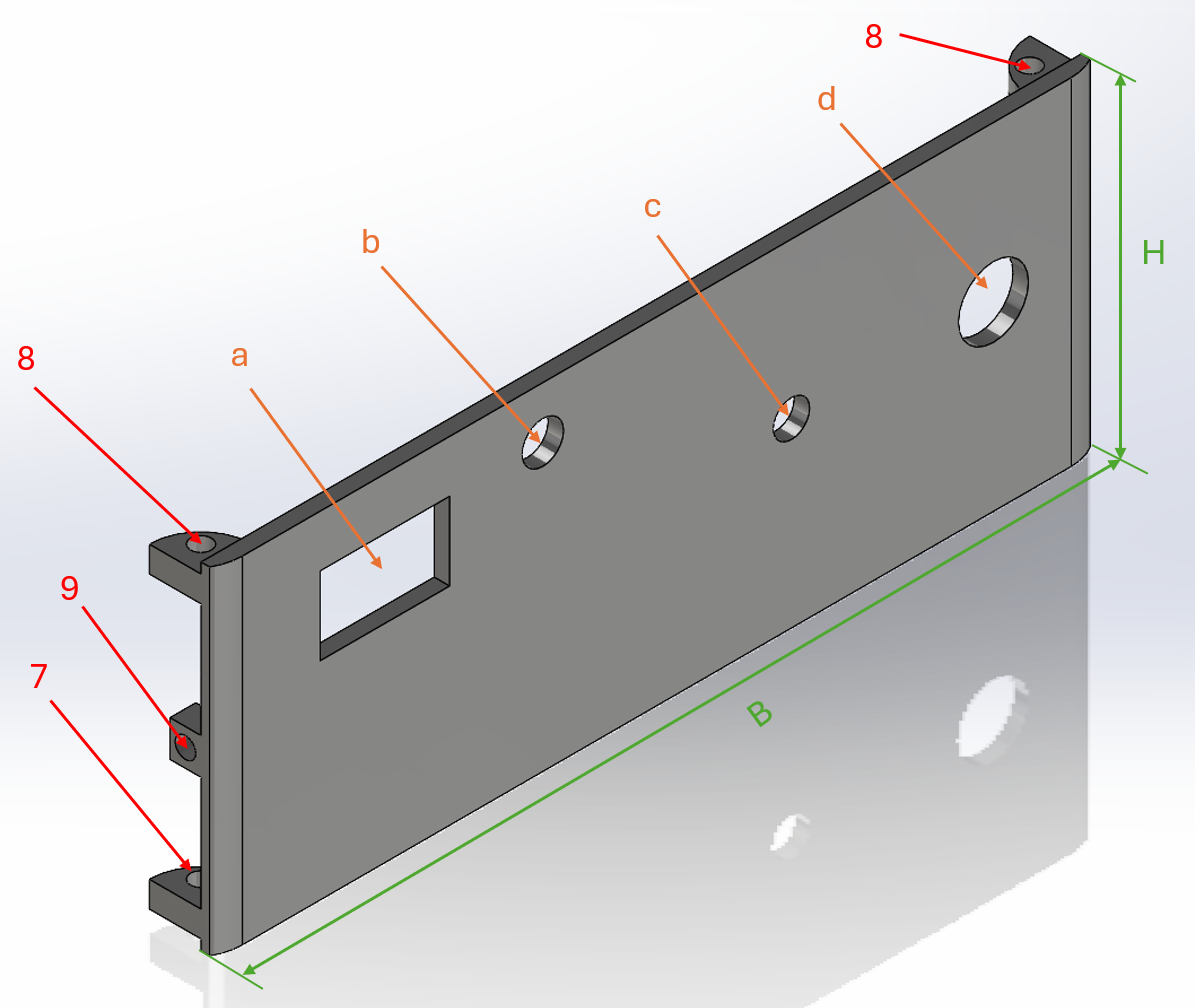
\includegraphics[width=\textwidth]{Images/Konstruktion/VorneK.png}
			\caption{Vorderplatte (Eigenaufnahme)} \label{VorneK}
		\end{center}
	\end{figure}

Die Seitenplatte Links wird an der Vorder- und Hinterplatte befestigt. Die Seitenplatte Links hat eine Länge von 177,32 \ mm, eine Höhe von 65 \ mm und eine Dicke von 5 \ mm, erkennbar in Abbildung \ref{SeiteLK}. Die Ecken sind mit einem Radius von 10 \ mm abgerundet. Die Bohrungen 10 und 11 sind der Tabelle \ref{BohrungenGK} aufgeführt. 


	\begin{figure}[H]
		\begin{center}
			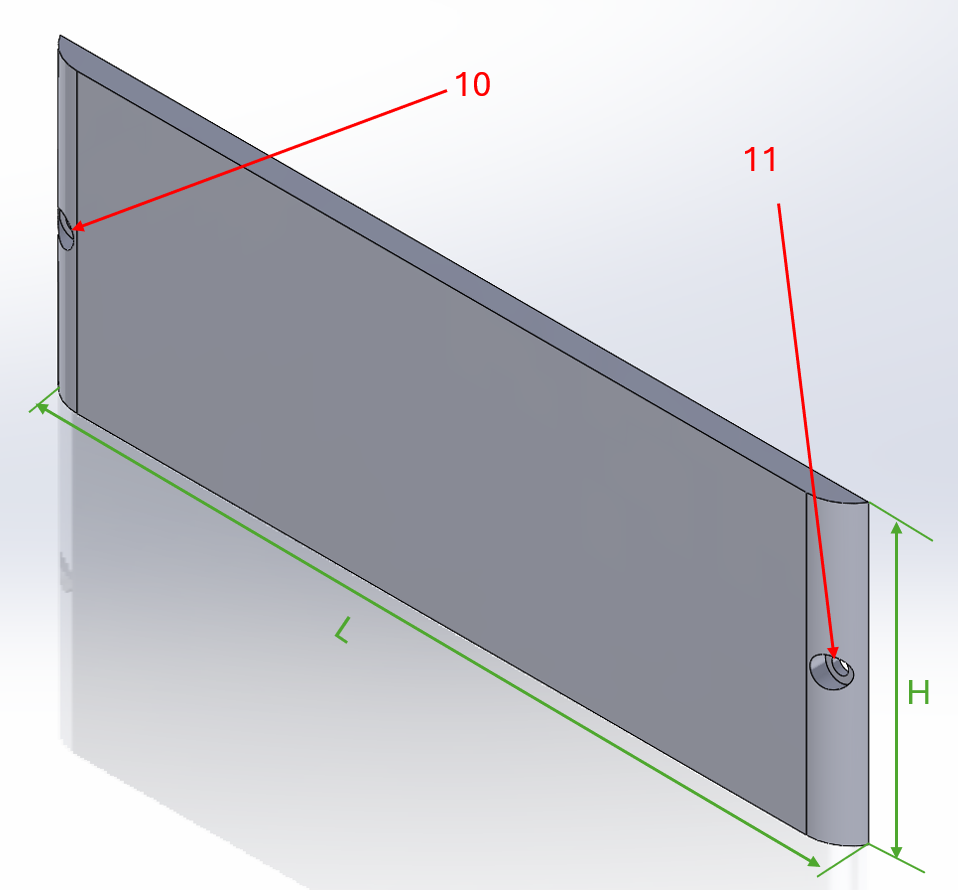
\includegraphics[width=\textwidth]{Images/Konstruktion/SeiteLK.png}
			\caption{Seitenplatte Links (Eigenaufnahme)} \label{SeiteLK}
		\end{center}
	\end{figure}

Die Hinterplatte wird an der Bodenplatte gefügt. Die Hinterplatte hat eine Breite B von 170 \ mm und eine Höhe H von 65 \ mm, erkennbar in Abbildung \ref{HinterK}. Der Kaltgerätestecker mit Artillerie-Wippschalter wird an der Außenseite der Rückplatte montiert (siehe Markierung e $30,5 \times 47 \ mm$  in Abb.\ref{HinterK}). Die Bohrungen 12 bis 15 sind der Tabelle \ref{BohrungenGK} aufgeführt.

	\begin{figure}[H]
		\begin{center}
			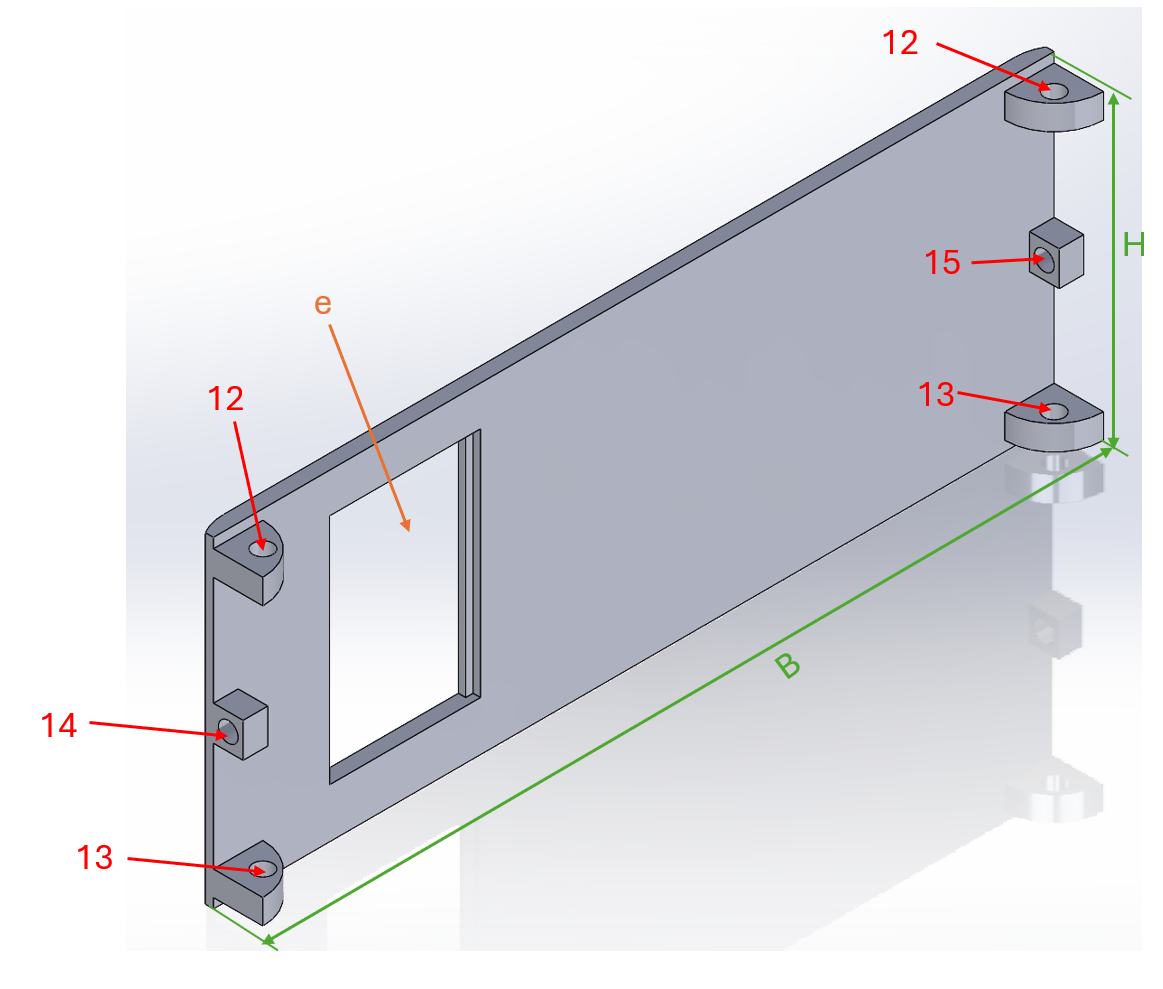
\includegraphics[width=\textwidth]{Images/Konstruktion/HinterK.png}
			\caption{Hinterplatte (Eigenaufnahme)} \label{HinterK}
		\end{center}
	\end{figure}

Die Seitenplatte Rechts wird an der Vorder- und Hinterplatte befestigt. Die Seitenplatte Rechts hat eine Länge von 177,32 \ mm, eine Höhe von 65 \ mm und eine Dicke von 5 \ mm, erkennbar in Abbildung \ref{SeiteLK}. Die Ecken sind mit einem Radius von 10 \ mm abgerundet. Für die Durchführung der Leitungen vom Schrittmotor und des Microschalters wurde eine Aussparung konstruiert (siehe Markierung f \O $ \ 13 \ mm$  in Abb.\ref{SeiteRK}). Die Bohrungen 16 und 17 sind der Tabelle \ref{BohrungenGK} aufgeführt. 


\begin{figure}[H]
	\begin{center}
		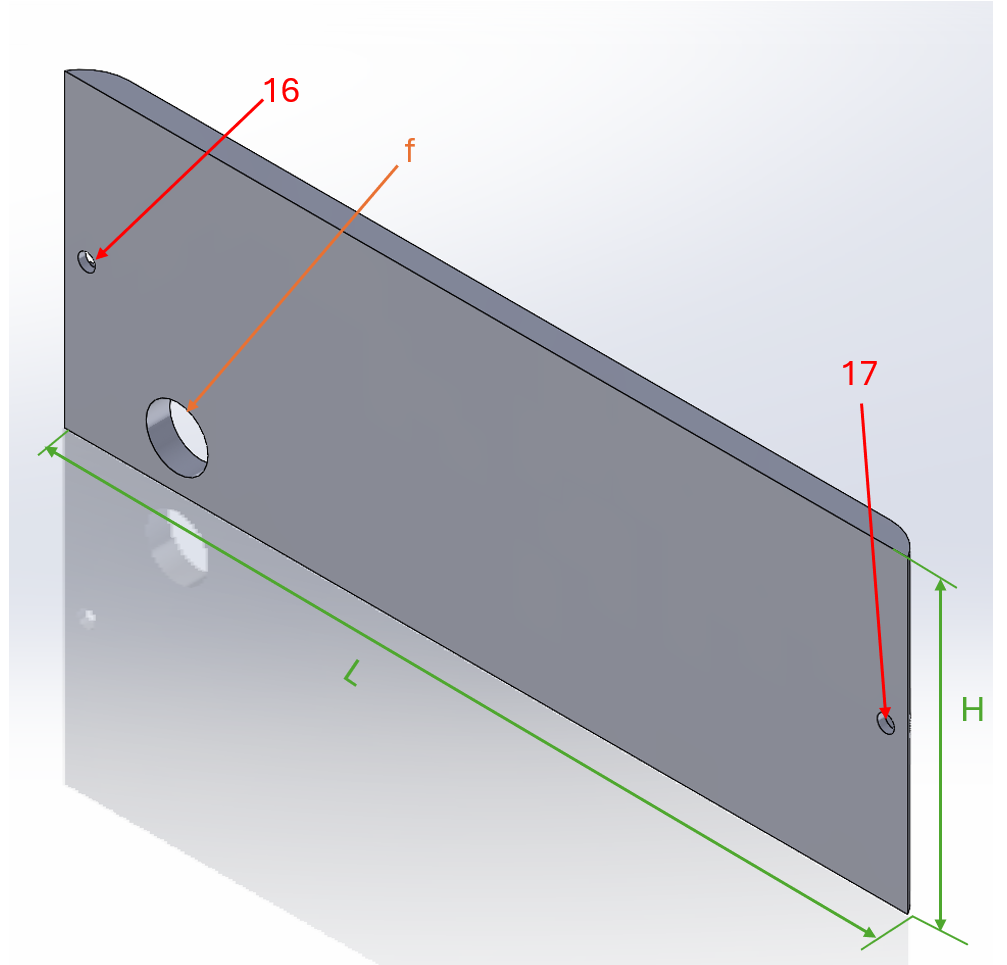
\includegraphics[width=\textwidth]{Images/Konstruktion/SeiteRK.png}
		\caption{Seitenplatte Rechts (Eigenaufnahme)} \label{SeiteRK}
	\end{center}
\end{figure}

Die Deckelplatte wird an der Vorder- und Hinterplatte befestigt. Die Deckelplatte hat ein Länge L von 180 mm und einer Breite B von 180 \ mm und einer Dicke von 7 \ mm, erkennbar in Abbildung \ref{DeckelK}. Die Ecken sind mit einem Radius von 10 \ mm abgerundet. Die Bohrungen 18 sind der Tabelle \ref{BohrungenGK} aufgeführt.

	\begin{figure}[H]
		\begin{center}
			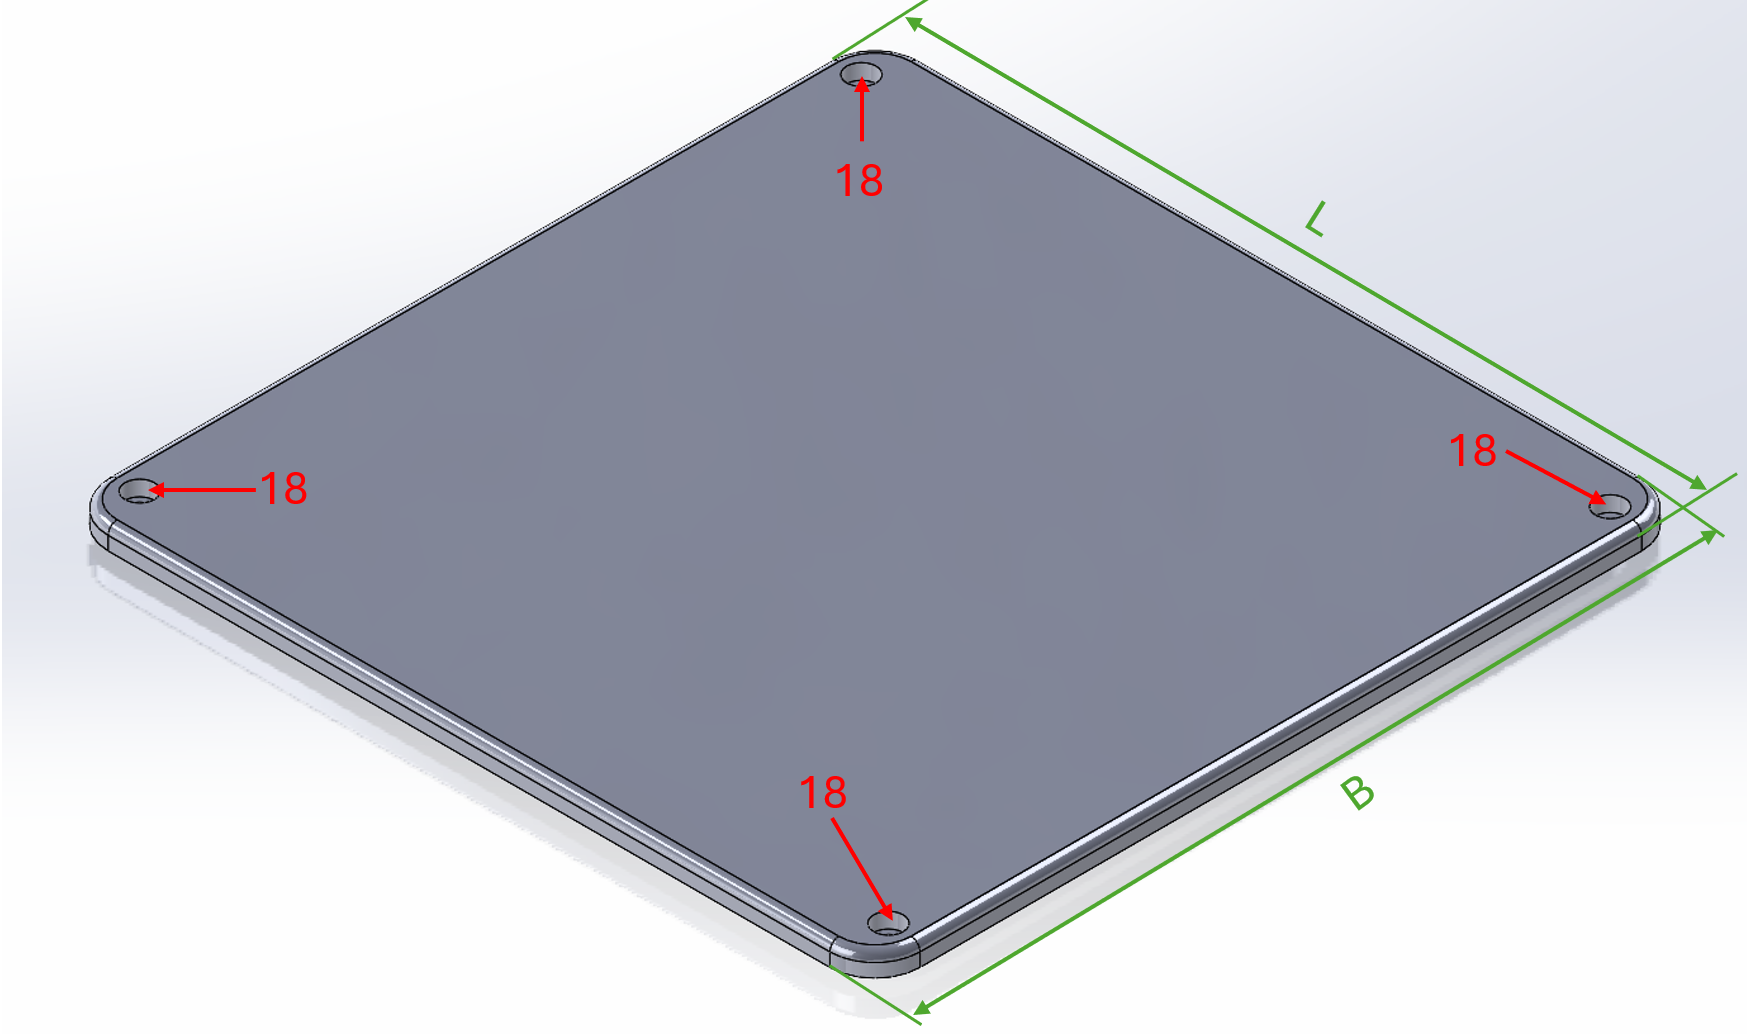
\includegraphics[width=\textwidth]{Images/Konstruktion/DeckelK.png}
			\caption{Deckelplatte (Eigenaufnahme)} \label{DeckelK}
		\end{center}
	\end{figure}
	
	
	\begin{figure}[H]
		\begin{center}
			\fontsize{8}{10}\selectfont
			\begin{tabularx}{\textwidth}{|p{0.4cm}|p{1.2cm}|X|X|X|X|} 
				\hline 
				\textbf{Nr.} & \textbf{\O} & \textbf{Beschreibung} \\ \hline
				1 & DIN912 M3 & Befestigung Schaltnetzteil an Bodenplatte \\ \hline
				2 & DIN912 M3 & Befestigung Tiny Maschine Learning Schield an Bodenplatte \\ \hline
				3 & DIN912 M3 & Fügen der Gehäuseteile an Bodenplatte  \\ \hline
				4 & DIN912 M3 & Befestigung Bodenplatte an Aluprofil \\ \hline
				5 & DIN912 M3 & Befestigung Schrittmotorsteuerung an Bodenplatte \\ \hline
				6 & DIN912 M3 & Befestigung des Halters für Spannungswandler an Bodenplatte \\ \hline
				7 & 4 \ mm & Bohrung für M3-Einpressmutter zur Befestigung Vorderplatte an Bodenplatte \\ \hline
				8 & 4 \ mm & Bohrung für M3-Einpressmutter zur Befestigung Vorderplatte an Deckelplatte \\ \hline
				9 & 4 \ mm & Bohrung für M3-Einpressmutter zur Befestigung Vorderplatte an Seitenplatte Links \\ \hline
				10& DIN912 M3 & Befestigung der Seitenplatte Links an Hinterplatte \\ \hline
				11& DIN912 M3 & Befestigung der Seitenplatte Links an Vorderplatte \\ \hline
				12& 4 \ mm & Bohrung für M3-Einpressmutter zur Befestigung Hinterplatte an Deckelplatte \\ \hline
				13& 4 \ mm & Bohrung für M3-Einpressmutter zur Befestigung Hinterplatte an Bodenplatte \\ \hline
				14& 4 \ mm & Bohrung für M3-Einpressmutter zur Befestigung Hinterplatte an Seitenplatte Links \\ \hline
				15& 4 \ mm & Bohrung für M3-Einpressmutter zur Befestigung Hinterplatte an Seitenplatte Rechts \\ \hline
				16& DIN912 M3 & Befestigung der Seitenplatte Rechts an Hinterplatte \\ \hline
				17& DIN912 M3 & Befestigung der Seitenplatte Rechts an Vorderplatte \\ \hline
				18& DIN912 M3 & Fügen der Gehäuseteile an Deckelplatte \\ \hline
			\end{tabularx}
			\captionof{table}{Bohrungen im Gehäuse}	\label{BohrungenGK}
		\end{center}
	\end{figure}

\section{Anbauteile}

Nachfolgend werden die Anbauteile in der Konstruktion beschrieben. 
In der Abbildung \ref{FlankeMotorK} zu erkennen, ist die Halterung für den Motor. Die Halterung hat ein Breite B von 50 \ mm und eine Höhe H von 70 mm und eine Dicke von 5 \ mm, erkennbar in Abbildung \ref{FlankeMotorK}. Sie enthält eine Aussparung für den Motor (siehe Markierung g Motor \O $ \ 22,5 \ mm$, Welle \O $ \ 6 \ mm$  in Abb.\ref{SeiteRK}). Die Halterung wird an dem Aluprofil montiert. Die Bohrungen 20 und 21 sind der Tabelle \ref{BohrungenAK} aufgeführt. 
 
	\begin{figure}[H]
		\begin{center}
			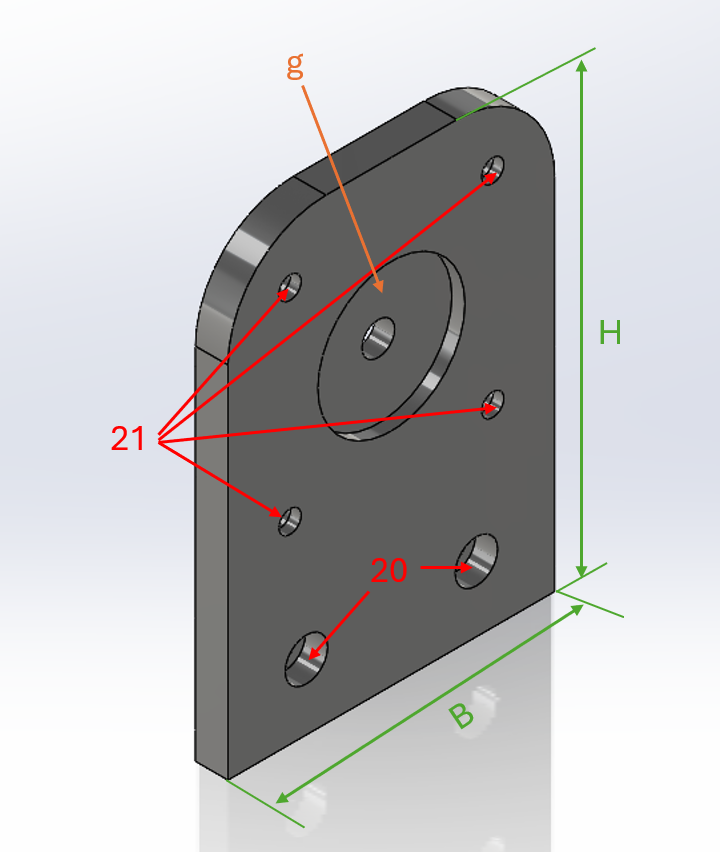
\includegraphics[width=\textwidth]{Images/Konstruktion/FlankeMotorK.png}
			\caption{Halterung für den Motor (Eigenaufnahme)} \label{FlankeMotorK}
		\end{center}
	\end{figure}
 
Die Halterung für die Welle hat eine Breite B von 50 \ mm und eine Höhe H von \ 70 mm und eine Dicke von 5 \ mm , erkennbar in Abbildung \ref{FlankeK}. Die Halterung besitzt eine Aussparung für die Welle (siehe Markierung h \O $ \ 5 \ mm$ in Abb.\ref{FlankeK}). Die Halterung wird an dem Aluprofil montiert. Die Bohrungen 22 sind der Tabelle \ref{BohrungenAK} aufgeführt.  
 
	\begin{figure}[H]
		\begin{center}
			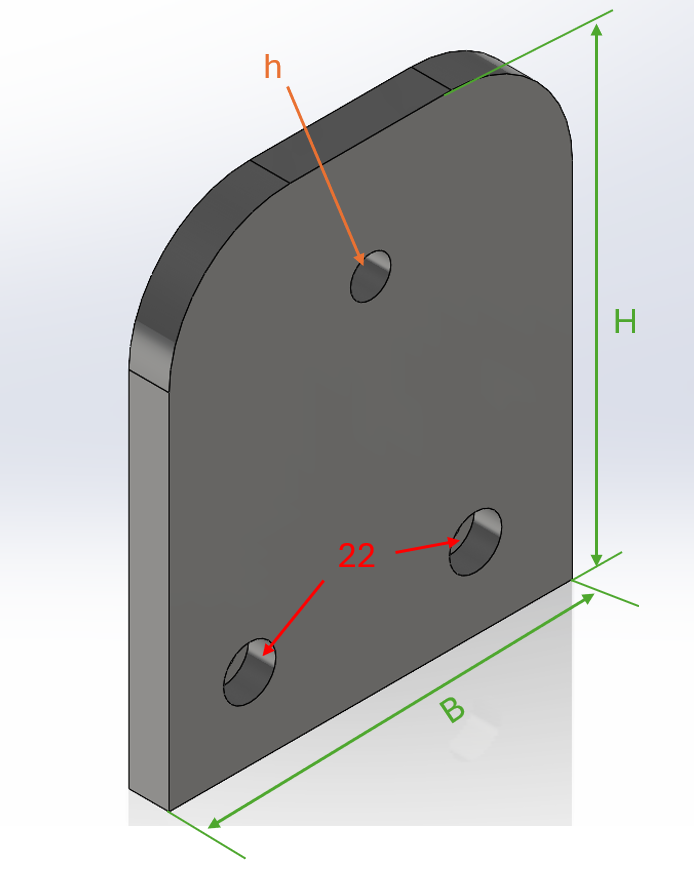
\includegraphics[width=\textwidth]{Images/Konstruktion/FlankeK.png}
			\caption{Halterung für die Welle (Eigenaufnahme)} \label{FlankeK}
		\end{center}
	\end{figure} 
	 
Der Griff zum Transportieren hat eine Breite B von 170 \ mm und eine Höhe H von 60 \ mm bei einer Dicke von 20 \ mm, die innere Spannweite Li beträgt 100 \ mm mit einer Höhe Hi von  50 \ mm , erkennbar in Abbildung \ref{GriffK}. Die Bohrungen 23 sind der Tabelle \ref{BohrungenAK} aufgeführt.  

	\begin{figure}[H]
		\begin{center}
			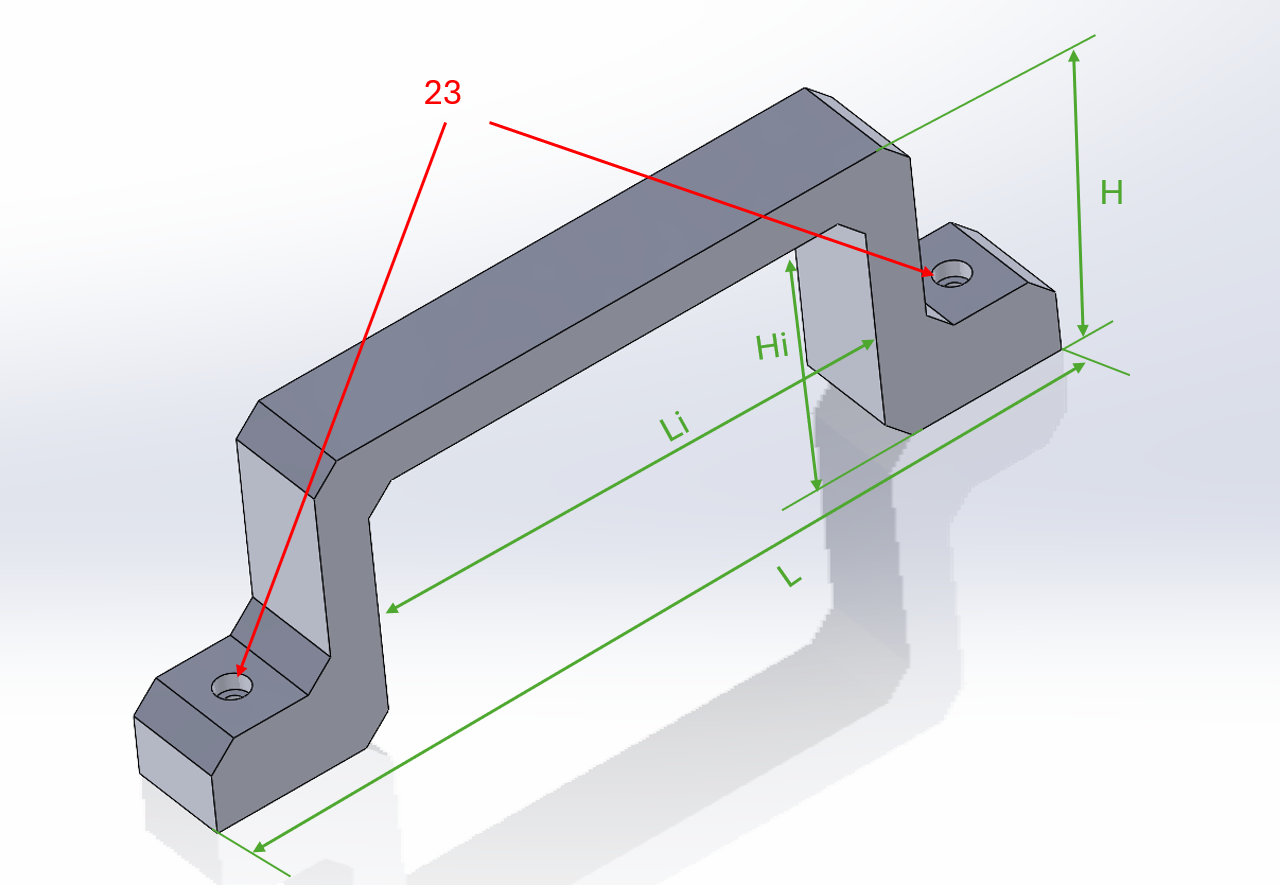
\includegraphics[width=\textwidth]{Images/Konstruktion/GriffK.png}
			\caption{Transportgriff (Eigenaufnahme)} \label{GriffK}
		\end{center}
	\end{figure}  

Der Drehknopf wird mittels einer DIN912 M3 Schraube auf dem Drehwinkel-Encoder befestigt. Der Drehknopf hat einen Durchmesser D von 32 \ mm und einer Länge von 20 \ mm. Der Drehknopf zeigt eine zahnförmige Kontur, erkennbar in Abbildung \ref{DrehKnopfK}. Die Bohrungen 24 sind der Tabelle \ref{BohrungenAK} aufgeführt.
	
	\begin{figure}[H]
		\begin{center}
			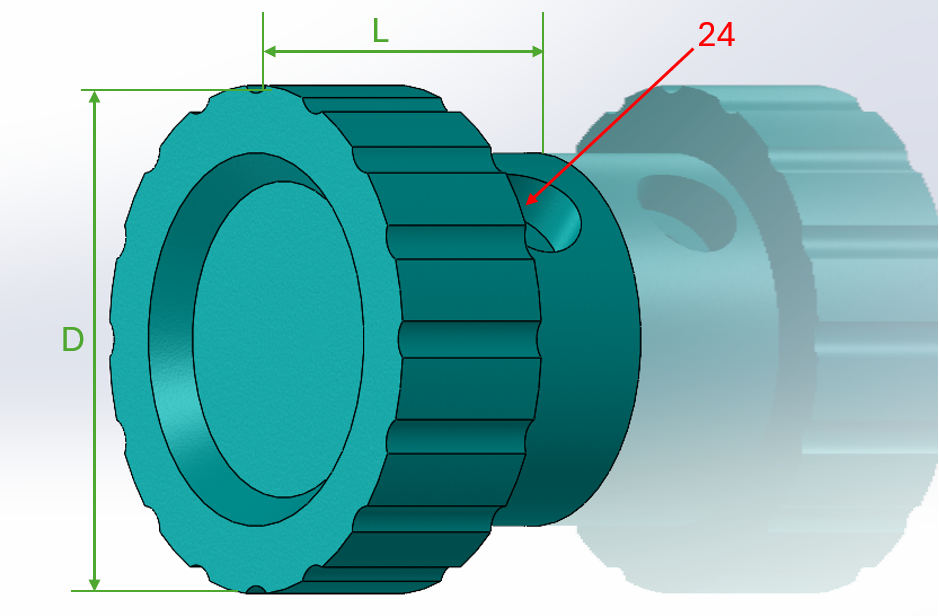
\includegraphics[width=\textwidth]{Images/Konstruktion/DrehKnopfK.png}
			\caption{Drehknopf (Eigenaufnahme)} \label{DrehKnopfK}
		\end{center}
	\end{figure}  

Der Anzeiger hat eine Breite B von 40 \ mm und eine Länge L von 50 \ mm, erkennbar in Abbildung \ref{AnzeigerK}. Der Pfeil (siehe Markierung i in Abb.\ref{AnzeigerK}) auf dem Anzeiger hat eine Tiefe von 35 \ mm. Die Bohrungen 25 und 26 sind der Tabelle \ref{BohrungenAK} aufgeführt.

	\begin{figure}[H]
		\begin{center}
			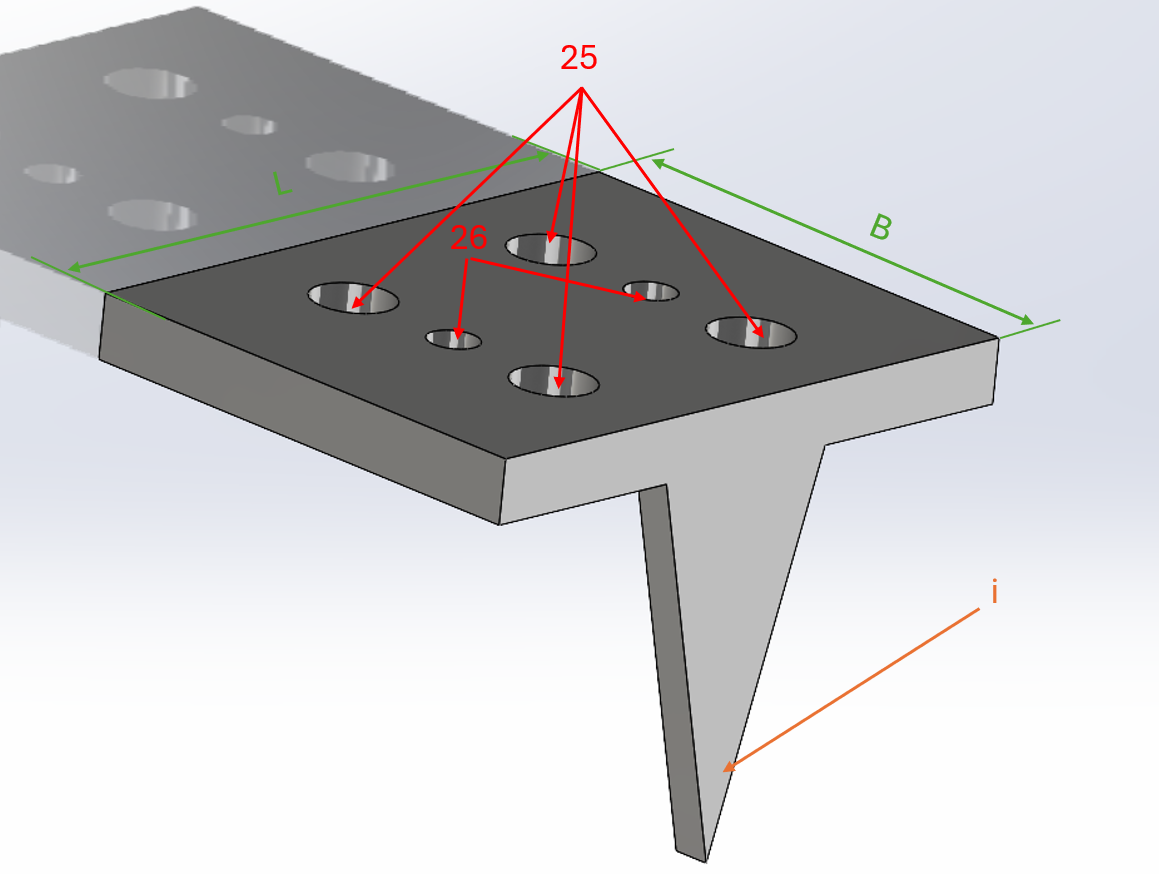
\includegraphics[width=\textwidth]{Images/Konstruktion/AnzeigerK.png}
			\caption{Anzeiger (Eigenaufnahme)} \label{AnzeigerK}
		\end{center}
	\end{figure}  
	 
	 \begin{figure}[H]
	 	\begin{center}
	 		\fontsize{8}{10}\selectfont
	 		\begin{tabularx}{\textwidth}{|p{0.4cm}|p{1.2cm}|X|X|X|X|} 
	 			\hline 
	 			\textbf{Nr.} & \textbf{\O} & \textbf{Beschreibung} \\ \hline
	 			20 & DIN912 M3 & Befestigung Motor an Flanke Halterung für Motor \\ \hline
	 			21 & DIN912 M3 & Befestigung Flanke Halterung für Motor an Aluprofil \\ \hline
	 			22 & DIN912 M3 & Befestigung Flanke an Aluprofil  \\ \hline
	 			23 & DIN912 M3 & Befestigung Griff an Aluprofil \\ \hline
	 			24 & DIN912 M3 & Befestigung Drehknopf mit Drehwinkel-Encoder \\ \hline
	 			25 & DIN912 M3 & Befestigung Anzeiger an Schlitten \\ \hline
	 			26 & 2,8 \ mm & Bohrung für M3-Einpressmutter zur Befestigung Riemen an Anzeiger \\ \hline
	 		\end{tabularx}
	 		\captionof{table}{Bohrungen der Anbauteile}	\label{BohrungenAK}
	 	\end{center}
	 \end{figure}

\section{3D-Druck mit PLA}
Die Einzelteile des Gehäuses sowie die Anbauteile wurden mit dem Anycubic Kobra 2 Neo gefertigt, wahrnehmbar in \ref{AKK2N}. Als Fertigungsmaterial wurde PLA gewählt. Das additve Verfahren eignet sich als kostengünstiges und schnelles Verfahren für den Prototypen-Bau. Für den Druck aller Einzelteile wurde c.a 0,5 kg Filament verbraucht. Der Preis für einen kg liegt bei ungefähr 20 €. Der längste Druck dauerte ca. 2,5 h. 

	 \begin{figure}[H]
	 	\begin{center}
	 		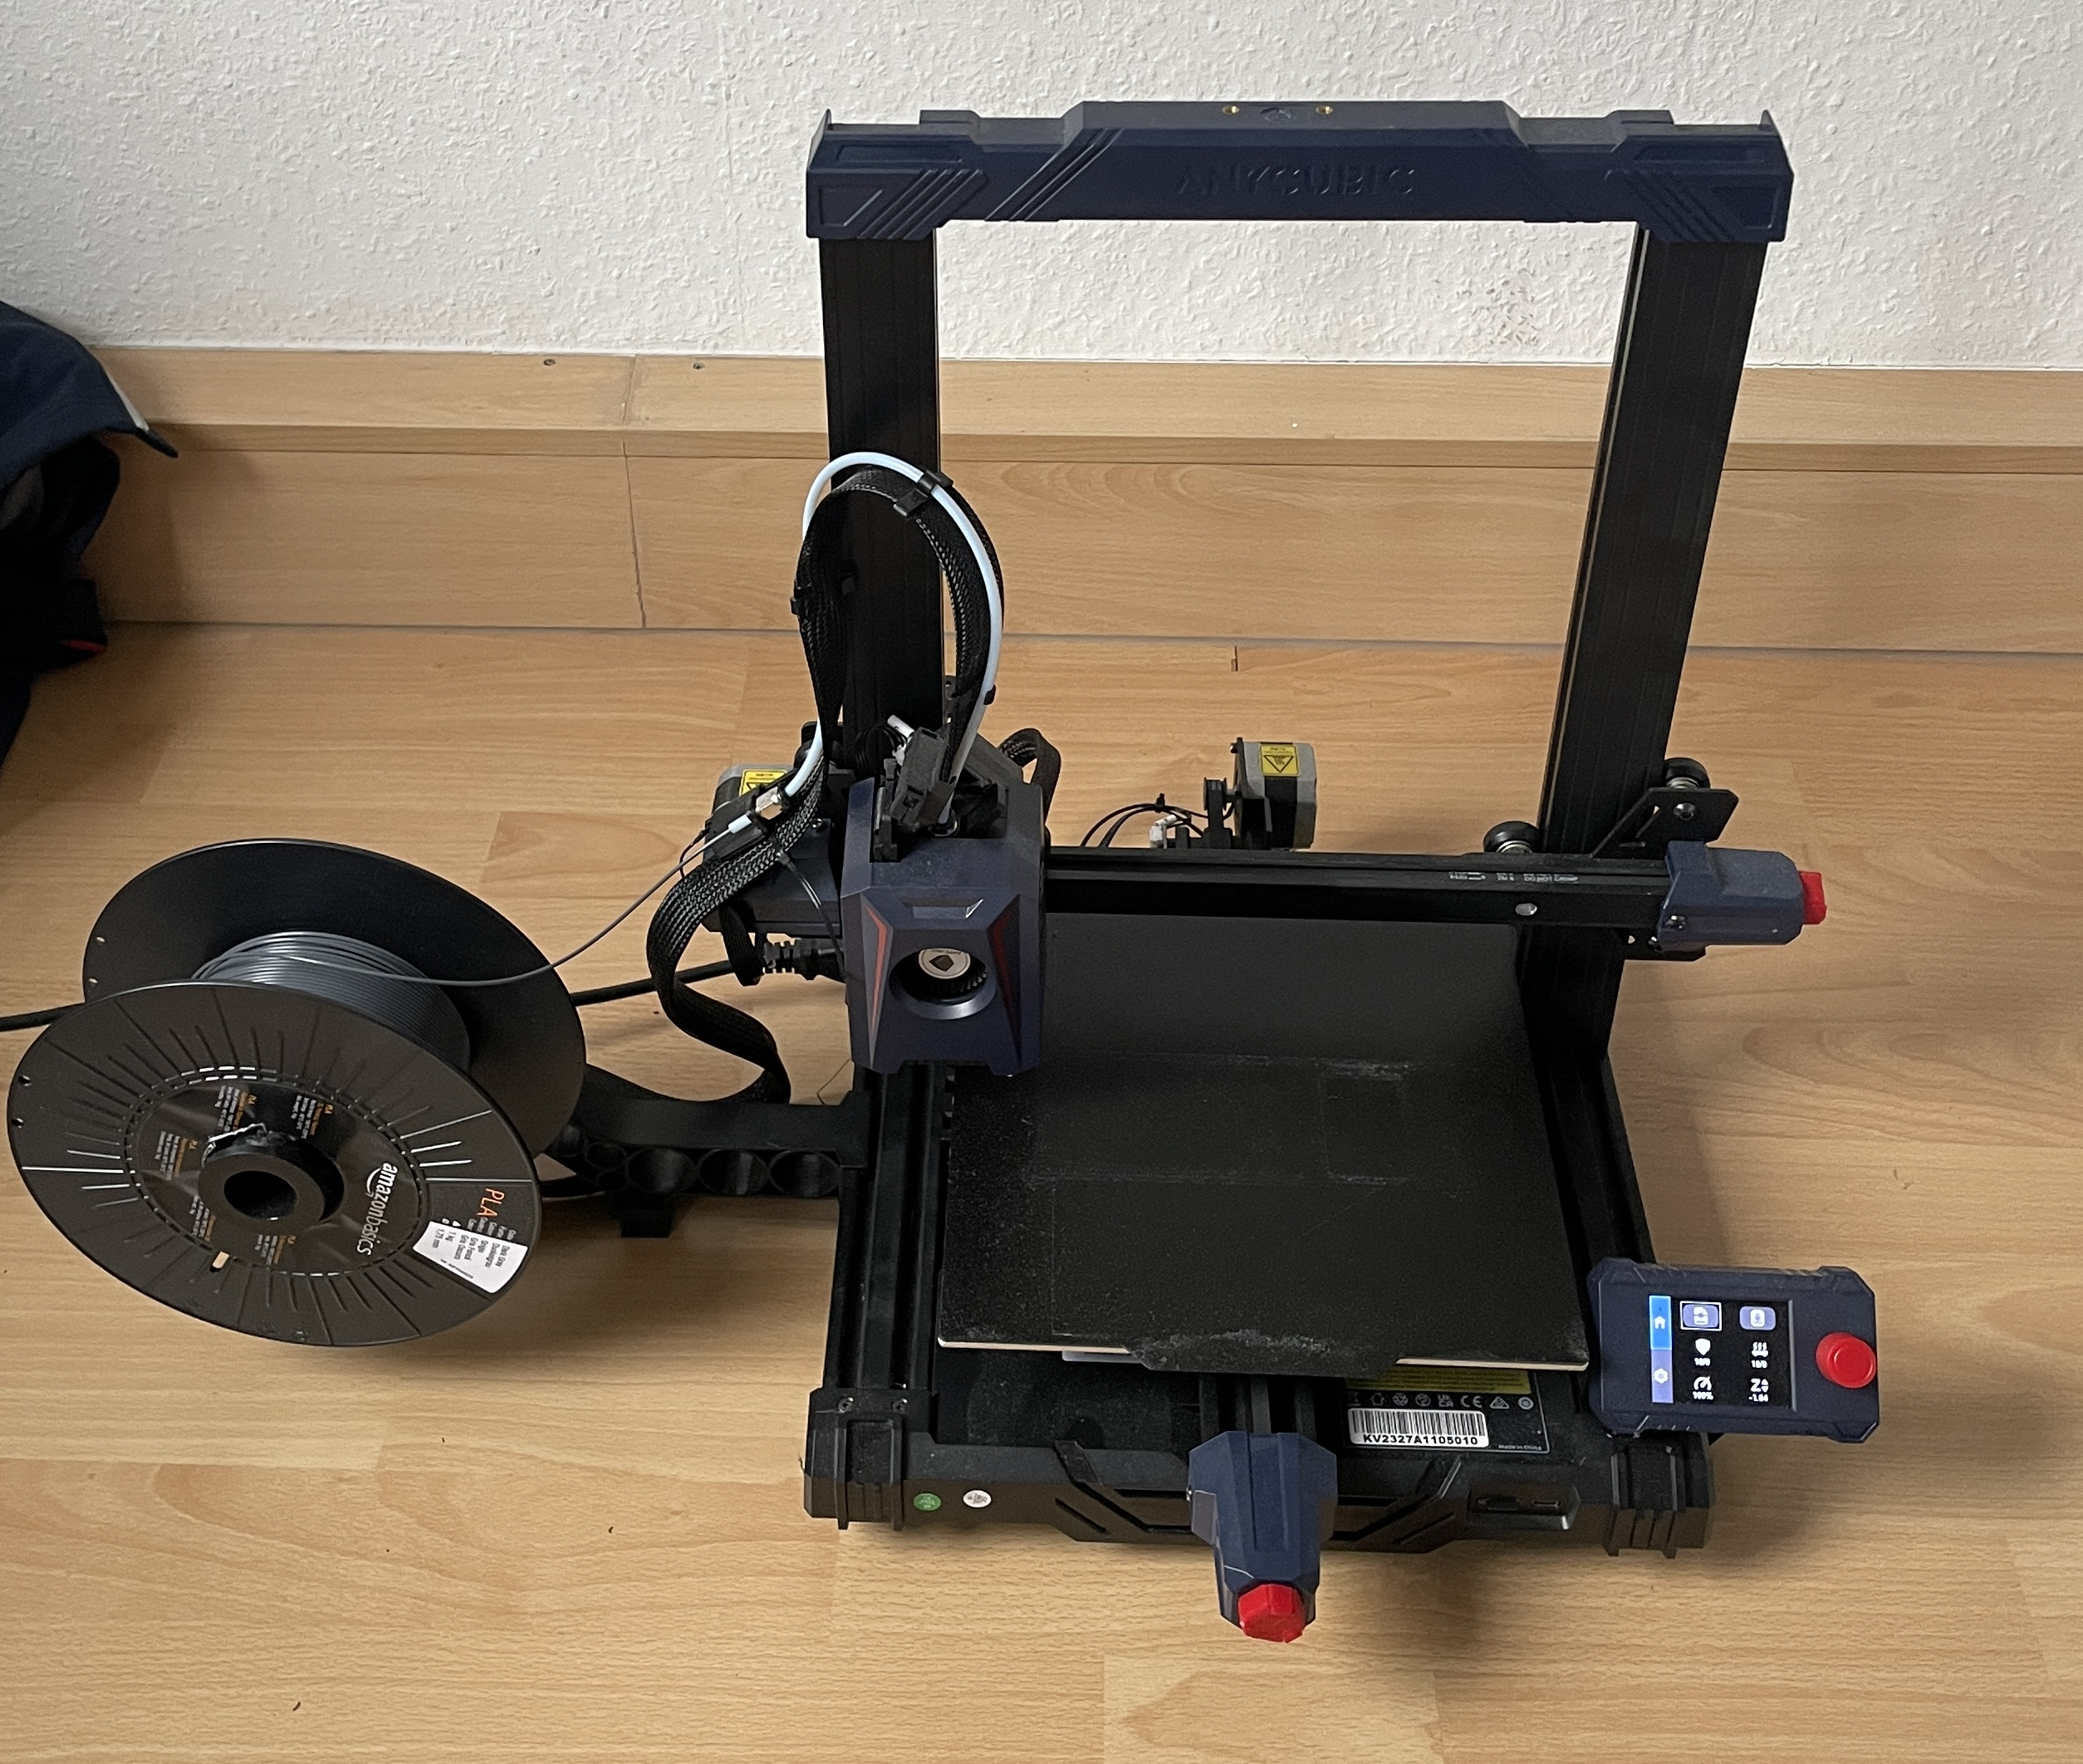
\includegraphics[width=\textwidth]{Images/Konstruktion/AKK2N.jpg}
	 		\caption{AnyKubic 2 Kobra Neo (Eigenaufnahme)} \label{AKK2N}
	 	\end{center}
	 \end{figure}  
